\section{Pre-Mitigation}
\label{sec:pre-mitigation}
Starting with version $0.5.0$, the BL-TMR toolflow supports pre-mitigated
top-level ports and design components. With previous versions of the tool,
pre-mitigated components had to be wired in manually which was a tedious and
error-prone process. The process is now much more automatic resulting in a
simpler design flow.

\subsection{Pre-mitigated top-level ports}
At times, it is desirable to use a single entity declaration for both a TMR and
non-TMR version of a design, with second and third domain top-level ports left
open in the non-TMR version. This can be accomplished by using pre-mitigated
top-level ports.

Consider a design with the following VHDL entity declaration:
\begin{verbatim}
entity compute_top is
  port (
    clk : in std_logic;
    rst : in std_logic;
    din : in std_logic_vector(7 downto 0);
    din1 : in std_logic_vector(7 downto 0);
    din2 : in std_logic_vector(7 downto 0);
    en : std_logic;
    en1 : std_logic;
    en2 : std_logic;
    dout : std_logic_vector(7 downto 0);
    dout1 : std_logic_vector(7 downto 0);
    dout2 : std_logic_vector(7 downto 0)
    );
end entity compute_top;
\end{verbatim}

Let us assume that in a non-TMR version of this design, we want to use the
\texttt{clk}, \texttt{rst}, \texttt{din}, \texttt{en}, and \texttt{dout} ports
as in Figure~\ref{fig:compute_top}.

\begin{figure}[htb]
\begin{center}
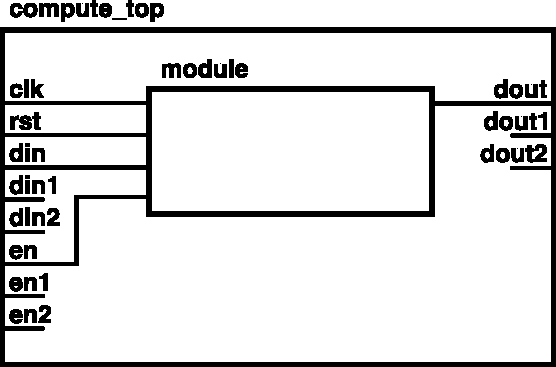
\includegraphics[width=3.5in]{compute_top.pdf}
\caption{compute\_top}
\label{fig:compute_top}
\end{center}
\end{figure}

In the TMR version we want the BL-TMR tool to triplicate the internals of the
design and wire up the second and third domains to the corresponding ports (i.e.
\texttt{din1} and \texttt{din2} correspond to the second and third domains for
\texttt{din}) as in Figure~\ref{fig:compute_top_tmr}.

\begin{figure}[htb]
\begin{center}
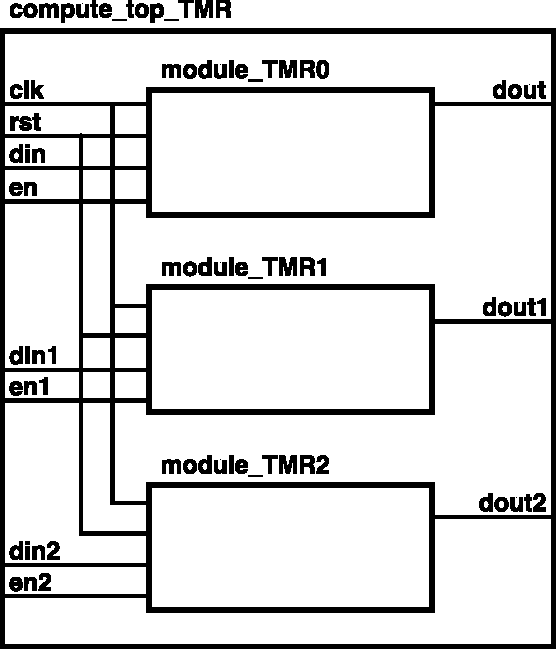
\includegraphics[width=3.5in]{compute_top_tmr.pdf}
\caption{compute\_top\_TMR}
\label{fig:compute_top_tmr}
\end{center}
\end{figure}

We can accomplish this by telling the tool about the port groupings (i.e.
\texttt{din}, \texttt{din1}, and \texttt{din2} form a port group). Each port
group has a replication type (one of \texttt{triplication} or
\texttt{duplication}) and a name. The name of a port group doesn't matter as
long as each port in the group has the same name. Each port in a port group has
an index. Each \texttt{triplication} port group must have three ports with
indices $0$, $1$, and $2$. Each \texttt{duplication} port group must have two
ports with indices $0$ and $1$. We tell the BL-TMR tool about our port groupings
through EDIF properties on the ports which can be generated using VHDL
attributes. The EDIF property should be named \texttt{port\_group} and should
be of type \texttt{string}. The format for the string is ``\texttt{<replication
type>:<port group name>:<port index>}''. For the \texttt{compute\_top} design
above, we would put the appropriate EDIF properties on the ports using the
following VHDL code:
\begin{verbatim}
entity compute_top is
  port (
    clk : in std_logic;
    rst : in std_logic;
    din : in std_logic_vector(7 downto 0);
    din1 : in std_logic_vector(7 downto 0);
    din2 : in std_logic_vector(7 downto 0);
    en : std_logic;
    en1 : std_logic;
    en2 : std_logic;
    dout : std_logic_vector(7 downto 0);
    dout1 : std_logic_vector(7 downto 0);
    dout2 : std_logic_vector(7 downto 0)
    );
	
    attribute port_group : string;

    attribute port_group of din : signal is "triplication:din:0";
    attribute port_group of din1 : signal is "triplication:din:1";
    attribute port_group of din2 : signal is "triplication:din:2";

    attribute port_group of en : signal is "triplication:en:0";
    attribute port_group of en1 : signal is "triplication:en:1";
    attribute port_group of en2 : signal is "triplication:en:2";

    attribute port_group of dout : signal is "triplication:dout:0";
    attribute port_group of dout1 : signal is "triplication:dout:1";
    attribute port_group of dout2 : signal is "triplication:dout:2";

end entity compute_top;
\end{verbatim}

Notice that the \texttt{clk} and \texttt{rst} signals do not have port group
attributes because we have chosen not to pre-triplicate these particular
signals. (We could still tell the BL-TMR tool to triplicate these ports, if
desired, by using the \texttt{--tmr\_p <port\_name>}). When the port group attributes
above are used in the VHDL code, the BL-TMR tool automatically wires the ports
to the appropriate domains after triplicating the design internals. Port groups can
also be used for pre-duplicated ports. A single design can mix
\texttt{triplication} and \texttt{duplication} port groups if desired.

\subsection{Pre-mitigated Components}
Pre-mitigated components are useful in situations where standard TMR with
bitstream scrubbing is not a sufficient mitigation strategy and alternative
mitigation strategies need to be implemented manually in certain portions of a
design before TMR is applied to the rest of the design. One such situation is
that of using a block RAM with a soft-core processor. Block RAMs are susceptible
to SEUs but bitstream scrubbing cannot correct errors in block BRAMs used as
RAM (not ROM) because there is no ``golden copy'' of the BRAM contents. A BRAM
scrubber can provide error correction in such a situation.

A TMR BRAM scrubber generally consists of three instances of a BRAM with
additional logic to repeatedly read the contents of the three BRAMs and correct
any bits where there is a discrepancy between the three copies. A BRAM scrubber
instantiates dual-ported BRAMs and uses one of the ports for scrubbing and
exposes the other port for normal access by the rest of the circuit.

Using a BRAM scrubber as a pre-mitigated component can simplify the process of
implementing TMR in the rest of the circuit. Consider a design that uses a
$4096$-bit single-port synchronous Block RAM with a port width of $4$
(RAMB$4$\_S$4$) as shown in Figure~\ref{fig:ramb4_s4}.

\begin{figure}[htb]
\begin{center}
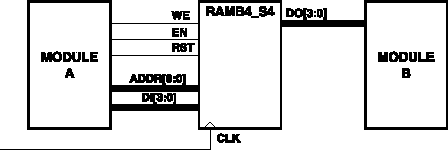
\includegraphics[scale=1]{ramb4_s4.pdf}
\caption{Design with Block RAM}
\label{fig:ramb4_s4}
\end{center}
\end{figure}

It is possible to develop a BRAM scrubber as a drop in replacement for the
single-port BRAM. Such a replacement would use three dual-ported BRAMs and
would expose all three TMR domains of one of the access ports to the rest of
the design as shown in Figure~\ref{fig:ramb4_s4_tmr}. For this example, we will
assume that we have developed such a scrubber.

\begin{figure}[htb]
\begin{center}
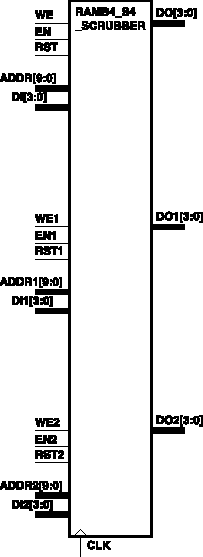
\includegraphics[scale=1]{ramb4_s4_tmr.pdf}
\caption{Block RAM Scrubber}
\label{fig:ramb4_s4_tmr}
\end{center}
\end{figure}

In this example, all signals have been triplicated except for the clock signal.
After replacing the original BRAM with the scrubber replacement we would have
the design shown in Figure~\ref{fig:ramb4_s4_tmr_design}. Notice that only the
first domain is wired for each signal since the rest of the design is still
untriplicated.

\begin{figure}[htb]
\begin{center}
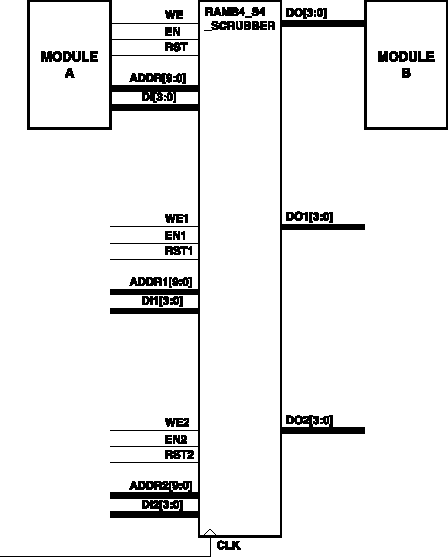
\includegraphics[scale=1]{ramb4_s4_tmr_design.pdf}
\caption{Design with Block RAM Scrubber}
\label{fig:ramb4_s4_tmr_design}
\end{center}
\end{figure}

By declaring port groups for the ports on the scrubber, we can tell the BL-TMR
tool how to wire up the unwired ports when the rest of the design gets
triplicated. As with pre-mitigated top-level ports, we do so by using VHDL
attributes. The entity declaration for our BRAM scrabber should be as follows:
\begin{verbatim}
entity RAMB4_S4_SCRUBBER
  port (
    WE : in std_logic;
    WE1 : in std_logic;
    WE2 : in std_logic;
    EN : in std_logic;
    EN1 : in std_logic;
    EN2 : in std_logic;
    RST : in std_logic;
    RST1 : in std_logic;
    RST2 : in std_logic;
    CLK : in std_logic;
    ADDR : in std_logic_vector(9 downto 0);
    ADDR1 : in std_logic_vector(9 downto 0);
    ADDR2 : in std_logic_vector(9 downto 0);
    DI : in std_logic_vector(3 downto 0);
    DI1 : in std_logic_vector(3 downto 0);
    DI2 : in std_logic_vector(3 downto 0);
    DO : out std_logic_vector(3 downto 0);
    DO1 : out std_logic_vector(3 downto 0);
    DO2 : out std_logic_vector(3 downto 0)
    );

  attribute port_group : string;

  attribute port_group of WE : signal is "triplication:WE:0";
  attribute port_group of WE1 : signal is "triplication:WE:1";
  attribute port_group of WE2 : signal is "triplication:WE:2";
  
  attribute port_group of EN : signal is "triplication:EN:0";
  attribute port_group of EN1 : signal is "triplication:EN:1";
  attribute port_group of EN2 : signal is "triplication:EN:2";

  attribute port_group of RST : signal is "triplication:RST:0";
  attribute port_group of RST1 : signal is "triplication:RST:1";
  attribute port_group of RST2 : signal is "triplication:RST:2";

  attribute port_group of ADDR : signal is "triplication:ADDR:0";
  attribute port_group of ADDR1 : signal is "triplication:ADDR:1";
  attribute port_group of ADDR2 : signal is "triplication:ADDR:2";

  attribute port_group of DI : signal is "triplication:DI:0";
  attribute port_group of DI1 : signal is "triplication:DI:1";
  attribute port_group of DI2 : signal is "triplication:DI:2";

  attribute port_group of DO : signal is "triplication:DO:0";
  attribute port_group of DO1 : signal is "triplication:DO:1";
  attribute port_group of DO2 : signal is "triplication:DO:2";
  
end entity RAMB4_S4_SCRUBBER;
\end{verbatim}

It should be noted that some care must be taken with synthesis tools in order
to preserve pre-mitigated components as separate components. Many synthesis
tools flatten some design hierarchy. When this happens to a pre-mitigated
component, the port declarations and port group properties are lost. The most
reliable way to prevent this is to leave pre-mitigated components as black
boxes in the main design and synthesize the pre-mitigated components separately
(making sure to disable IO buffer insertion). This results in a main EDIF
file for the top design component and a separate EDIF file for each
pre-mitigated component. The BL-TMR tool can merge the black boxes into the main
design while preserving port group properties if all of the EDIF files are
placed in the same directory or their paths are indicated using the appropriate
commandline options.

When the BL-TMR tool is used to apply TMR to the design in
Figure~\ref{fig:ramb4_s4_tmr_design} with the port group attributes shown above,
the resulting design has all of the ports wired up to the appropriate domains
as shown in Figure~\ref{fig:ramb4_s4_tmr_result}.

\begin{figure}[htb]
\begin{center}
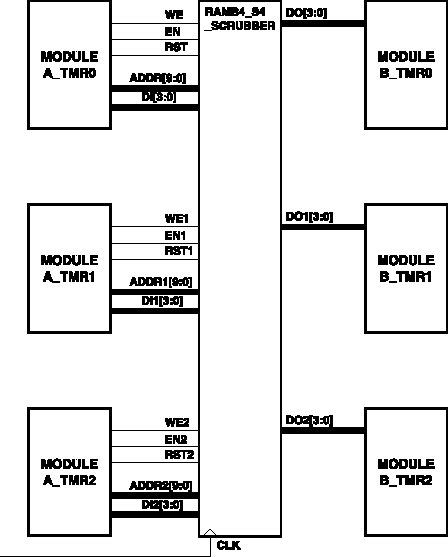
\includegraphics[scale=1]{ramb4_s4_tmr_result.pdf}
\caption{Triplicated Design with Block RAM Scrubber}
\label{fig:ramb4_s4_tmr_result}
\end{center}
\end{figure}

\subsection{Implementation Issues}
\subsubsection{VHDL Open Ports}
In order to create a design with unconnected ports such as that shown in
Figure~\ref{fig:ramb4_s4_tmr_design}, it is necessary to leave the unused
(i.e. second and third domain) ports \texttt{open} in the VHDL component
instantiation statement. Synthesis tools generally wire \texttt{open} ports
with no default value specified to \texttt{GND}. The BL-TMR tool removes any
connections on second and third domain ports of pre-mitigated components before
wiring them to the rest of the design in order to prevent input ports from
being driven by \texttt{GND} in addition to their correct drivers.

\subsubsection{Proprietary Pre-mitigated Cores}
Some core formats such as .ngc are proprietary and cannot be read by the BL-TMR
tool. When a pre-mitigated core is in a proprietary format, it can still be
used, however, because the BL-TMR tool simply works on the black box definition
of the core. All appropriate connections to the black box will be made and the
core can be merged in by proprietary tools after running the BL-TMR tool. The
only difficulty with this process is that any \texttt{port\_group} properties for
pre-mitigated proprietary cores must be inserted into the black box cell
definition in the main EDIF file manually because VHDL has no means of putting
attributes on component declaration ports.
